\documentclass{article}
\usepackage[utf8]{inputenc}
\usepackage{graphicx}

\author{Bijan Varjavand}
\title{LabNotebook}
\date{February 14, 2017}

\begin{document}

\maketitle

\section{Objectives}

The goal this lab was to measure differences between temperature and conductivity for a silicon wafer.

\section{Setup}

Silicon wafers of specific conductivities had to be made. Our group went to the microfabrication lab on campus to create electrode leads on the samples for ourselves to use.
\subsection{Materials}

Silicon, doped some unspecified amount. Our wafer was 9cm x 1.9cm with a 0.05cm thickness.
\subsection{Tools}

Our group used power sources and multimeters for our measurements, as well as a thermocouple and a furnace.
\section{Procedure}

We added a thermocouple, wrapping it around the sample. This was to measure voltage, which we can convert to
temperature. A diagram of this setup is shown in Lab 1B. It is the same except for us only attaching our probes to the exposed parts of the wafer.\\

We also modulated the distance between our probes since we had a few different sections which we exposed.

\section{Results}

The figure that was generated with the data is shown below. We were also able to collaborate with different groups to get data from differently doped wafers.

\begin{figure}[h!]
\centering
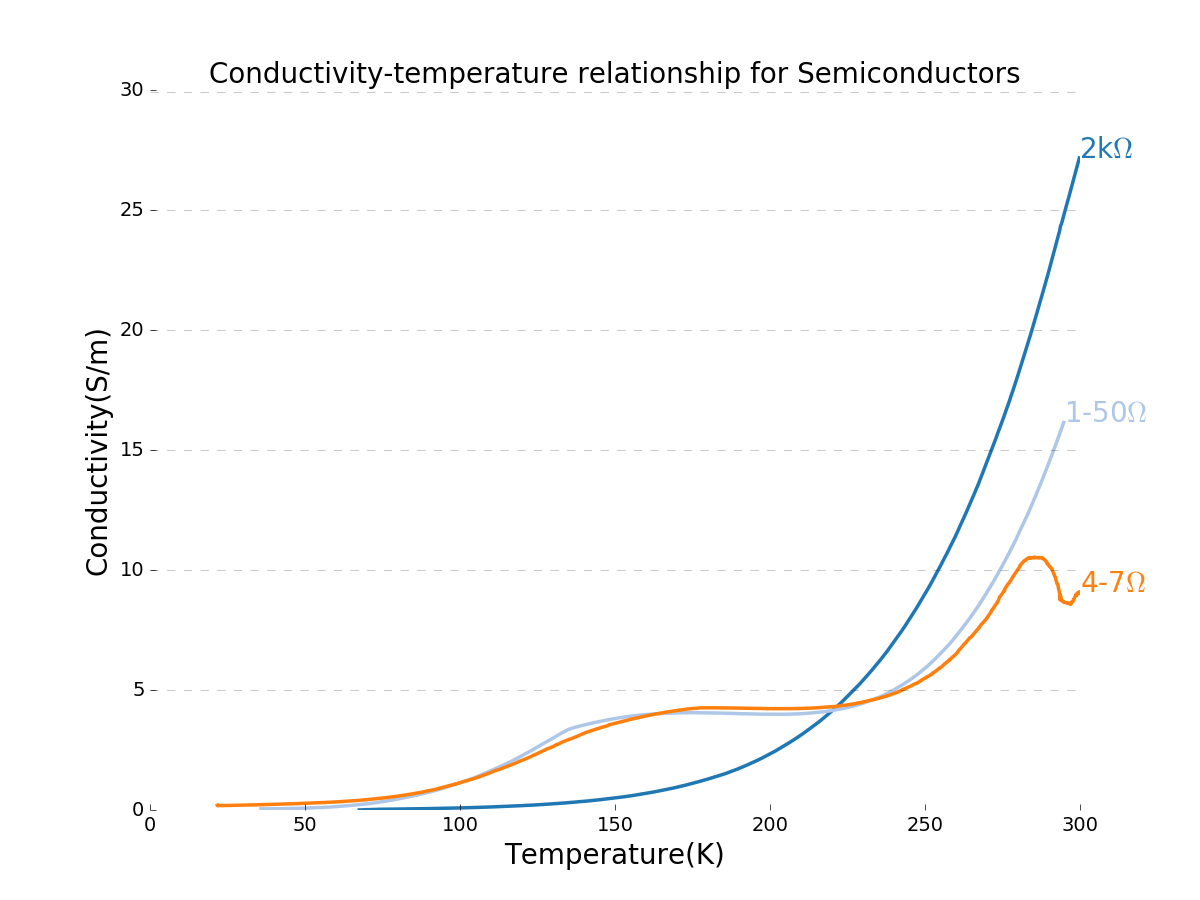
\includegraphics[scale=0.4]{semiconductors2.png}
\end{figure}

\section{Observations}

Matthiessen's Rule is followed properly by the data. The higher doped silicon (lower resistance) showed greater conductivity initially, but at higher temperatures only act as impurities which decrease conductivity.

\end{document}